% vim: spelllang=es spell
\documentclass{article}
\usepackage[margin=32mm]{geometry}
\usepackage{indentfirst}
\usepackage{amsmath}
% \usepackage{amssymb}
% \usepackage{enumitem}
\usepackage{graphicx}
\graphicspath{ {./hecho/} }
\title{Estructra de Computadores \\
	Práctica 1
	\medbreak
	\large Sumadores y Multiplicadores \\
	\bigbreak}
\author{Rubén López Singla\\
	\texttt{ruben.lopez@estudiants.urv.cat}
}
\date{\bigbreak $2023/03/15$}
\begin{document}

\maketitle

\newpage
\subsection*{Introducción}
En este informe documentamos las tareas realizadas en la primera práctica de Estructuras de Computadores. 

\renewcommand*\contentsname{Índice}
\setcounter{secnumdepth}{0} % sections are level 1 % no quiero numeros en las secciones ("FASE 5. -- TAREA 14" queda raro...)
\tableofcontents


\newpage
\section{FASE 1: Sumadores HA, FA}
	\subsection{TAREA 1: Half Adder}
		\subsubsection*{Especificación}
		Realizad el circuito digital Half Adder (HA) de 1 bit mostrado en la siguiente figura.
		Suponed que los retardos de las puertas lógicas utilizadas son AND=4T y XOR=5T. (0.125P)

		\subsubsection*{Diseño}
		Se ha seguido la implementación mostrada en la imagen de ejemplo.


		\subsubsection*{Implementación}
		 \begin{figure}[ht]
		 	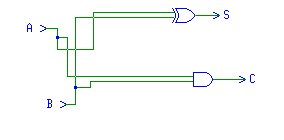
\includegraphics[width=0.8\linewidth]{HA}
			\centering
		 \end{figure}


		\subsubsection*{Juego de pruebas}
		
		\begin{table}[ht]
			\begin{center}
				\begin{tabular}{| c | c | c | c |}
					\hline
					Tipo de prueba & Operación & Resultado esperado & Funciona \\ \hline
					
					Suma & 1+0 & S=1 C=0 & Si \\ \hline
					Suma con carry & 1+1 & S=0 C=0 & Si \\ \hline
				\end{tabular}
				\caption Juego de pruebas
			\end{center}
		\end{table}

		\subsubsection*{Análisis de resultados}
		El circuito funciona adecuadamente.


	\subsection{TAREA 2: Full Adder}
		\subsubsection*{Especificación}
		Realizad el circuito digital Full Adder (FA) de 1 bit con acarreo de entrada utilizando
		sumadores Half Adders (HA) de 1 bit e indicad los tiempos de retardo y el área utilizada. Suponed
		que los retardos de las puertas lógicas utilizadas son de AND=4T, OR=4T y XOR=5T. (0.125P)

		\subsubsection*{Diseño}
		Se ha seguido la implementación mostrada en la imagen de ejemplo.


		\subsubsection*{Implementación}
		 \begin{figure}[ht]
		 	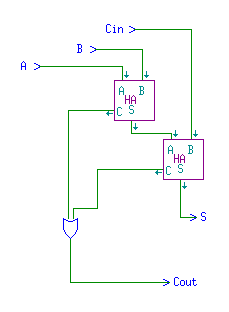
\includegraphics[width=0.8\linewidth]{FA}
		 	\centering
		 \end{figure}


		\subsubsection*{Juego de pruebas}
			\begin{table}[ht]
			\begin{center}
				\begin{tabular}{| c | c | c | c |}
					\hline
					Tipo de prueba & Operación & Resultado esperado & Funciona \\ \hline
					
					Suma & 1+0 Ci=0 & S=1 C=0 & Si \\ \hline
					Suma con carry & 1+1 Ci= 1 & S=1 C=1 & Si \\ \hline
				\end{tabular}
				\caption Juego de pruebas
			\end{center}
		\end{table}

		\subsubsection*{Análisis de resultados}
		El circuito funciona correctamente. Tiene un área de 34 unidades y un tiempo de retardo de 10T en la suma y 13T en el carry.


	\subsection{TAREA 3: Implementación alternativa al Full Adder}
		\subsubsection*{Especificación}
		Realizad una implementación alternativa al mismo circuito Full Adder (FA) de 1 bit con acarreo de entrada y comparad los tiempos de retardo y área con la solución anterior.
		Suponed los mismos retardos de las puertas lógicas utilizadas en la tarea anterior. (0.25P)

		\subsubsection*{Diseño}
		El diseño de este Full Adder se ha llevado a cabo calculando la tabla de la verdad de las diferentes partes del circuito y implementando los resultados de estas. Se ha utilizado el retardo por defecto de TkGate.


		\subsubsection*{Implementación}
		 \begin{figure}[ht]
		 	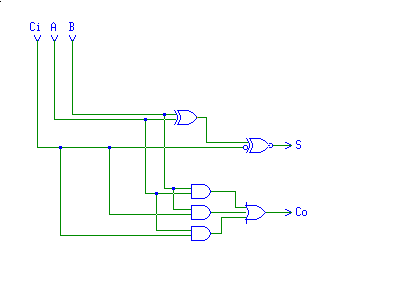
\includegraphics[width=0.8\linewidth]{FAA}
			\centering
		 \end{figure}


		\subsubsection*{Juego de pruebas}
		\begin{table}[h]
			\begin{center}
				\begin{tabular}{| c | c | c | c |}
					\hline
					Tipo de prueba & Operación & Resultado esperado & Funciona \\ \hline
					Suma & 1+0 Ci=0 & S=1 C=0 & Si \\ \hline
					Suma con carry & 1+1 Ci= 1 & S=1 C=1 & Si \\ \hline
			
				\end{tabular}
				\caption Juego de pruebas
			\end{center}
		\end{table}


		\subsubsection*{Análisis de resultados}
		El circuito funciona adecuadamente. El área es mayor a la de la implementación anterior con 42u, manteniendo el tiempo de suma en 10T pero reduce el tiempo de retardo del carry a 8.

\section{FASE 2: Sumadores CPA}
	\subsection{TAREA 4: Carry Propagate Adder}
		\subsubsection*{Especificación}
		Realizad el circuito digital Carry Propagate Adder (CPA) de 4 bits que se muestra en la
		siguiente figura e indicad y formulad los tiempos de retardo y el área utilizada. Asumid el Full
		Adder (FA) de 1 bit considerado en la Tarea 2. (0.5P)


		\subsubsection*{Diseño}
		Se ha seguido la implementación mostrada en las imagenes de ejemplo.

		\subsubsection*{Implementación}
		 \begin{figure}[ht]
			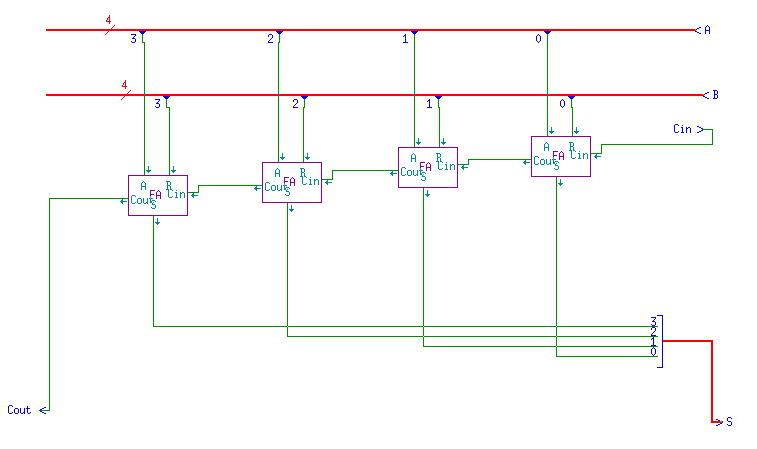
\includegraphics[width=0.8\linewidth]{CPA}
		 	\centering
		 \end{figure}


		\subsubsection*{Juego de pruebas}
		\begin{table}[h]
			\begin{center}
				\begin{tabular}{| c | c | c | c |}
					\hline
					Tipo de prueba & Operación & Resultado esperado & Funciona \\ \hline
					
					Suma & 3+2 Ci=1 & 6 Co=0 & Si \\ \hline
					Suma con carry & 7+8 Ci=1 & 0 Co=1 & Si \\ \hline
				\end{tabular}
				\caption Juego de pruebas
			\end{center}
		\end{table}



		\subsubsection*{Análisis de resultados}
		El circuito funciona adecuadamente. Tiene un área utilizada de 136 unidades y un tiempo de retardo de 37T para el carry y 34T para la suma.

	\subsection{TAREA 5: Implementación alternativa al CPA}
		\subsubsection*{Especificación}
		Realizad el circuito digital Carry Propagate Adder (CPA) de 4 bits que se muestra en la siguiente figura e indicad los tiempos de retardo y el área utilizada.
		Asumid el Full Adder (FA) de 1 bit considerado en la Tarea 3. (0.5P)


		\subsubsection*{Diseño}
		Se ha implementado el circuito igual que el diseño anterior, pero cambiando el Full Adder utilizado.


		\subsubsection*{Juego de pruebas}
		\begin{table}[h]
			\begin{center}
				\begin{tabular}{| c | c | c | c |}
					\hline
					Tipo de prueba & Operación & Resultado esperado & Funciona \\ \hline
						
					Suma & 3+2 Ci=1 & 6 Co=0 & Si \\ \hline
					Suma con carry & 7+8 Ci=1 & 0 Co=1 & Si \\ \hline
	
				\end{tabular}
				\caption Juego de pruebas
			\end{center}
		\end{table}



		\subsubsection*{Análisis de resultados}
		El circuito funciona adecuadamente. Tiene un área de 168 unidades, ya que estos Full Adders son de mayor área, y un tiempo de retardo de 32T en carry y 28T en la suma.
	\subsection{TAREA 6: Tiempos de retardo del CPA}
		\subsubsection*{Especificación}
		Indicad las fórmulas que describen los tiempos de retardo del circuito digital Carry Propagate Adder (CPA) de 4 bits implementado en las tareas anteriores.
		Aplicando esa fórmula, mostrad los tiempos de retardo que introduciría un CPA de 8 bits, 16 bits, 32 bits, 64 bits y 128 bits para cada una de las dos posibles implementaciones de Full Adder (FA) de 1 bit consideradas en las tareas anteriores \textbf{(0.75P)}

		\subsubsection*{Diseño}
		El retardo del CPA depende de lo que tarde en propagarse el Carry. En el primer diseño, tenemos que el primer carry tarda 13T en generarse, y la primera suma ocurrirá en paral·lelo a la propagación del carry. $ TC(n) = 13 + (n-1 bits) * (13-5) $ y que $ TS(n) = 13 + (n-2)*8 + 8 $
		
		En el segundo diseño, encontrariamos que $ TC(n) = 8 + (n-1 bits)*4 $, y que $ TS(n) = 8 + (n-2)*4+4 $	
	\subsection{TAREA 7: CPA de 16 bits}
		\subsubsection*{Especificación}
		Realizad un circuito digital Carry Propagate Adder (CPA) de 16 bits e indicad y
		formulad los tiempos de retardo y el área utilizada. Utilizad para esta implementación el circuito
		Carry Propagate Adder (CPA) de 4 bits implementado en la Tarea 4. (0.75P)

		\subsubsection*{Diseño}
		Imitando los diseños anteriores, hemos implementado este circuito con varios CPA de 4 bits en cadena.

		\subsubsection*{Implementación}
		 \begin{figure}[ht]
			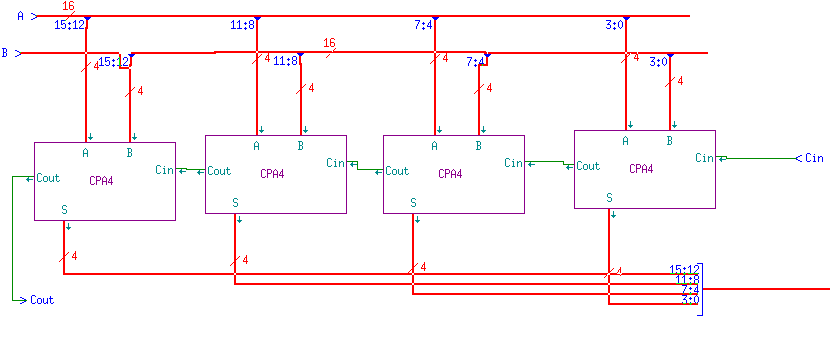
\includegraphics[width=0.8\linewidth]{CPA16}
		 	\centering
		 \end{figure}



		\subsubsection*{Juego de pruebas}
		\begin{table}[h]
			\begin{center}
				\begin{tabular}{| c | c | c | c |}
					\hline
					Tipo de prueba & Operación & Resultado esperado & Funciona \\ \hline
						
					Suma & 16+16 Ci=1 & 33 Co=0 & Si \\ \hline
					Suma con carry & 0xffff + 0xa & 9 Co=1 & Si \\ \hline
	
				\end{tabular}
				\caption Juego de pruebas
			\end{center}
		\end{table}



		\subsubsection*{Análisis de resultados}
		El circuito funciona adecuadamente. Tiene un área de 544 y un tiempo de retraso de 133T. Hace falta notar que el TKGate crashea al intentar calcular el camino crítico.  

	
	\subsection{TAREA 8}
		\subsubsection*{Especificación}
		Realizad un circuito digital restador de 16 bits e indicad los tiempos de retardo y el área
		utilizada. (0.5P)

		\subsubsection*{Diseño}
		En binario, el resutado de la suma es igual al resultado de restar. Entonces, la única diferencia es el "carry", que pasamos a llamar borrow, que se invertira en este circuito del Half Substractor en referencia al Half Adder.


		\subsubsection*{Implementación}
		 \begin{figure}[ht]
			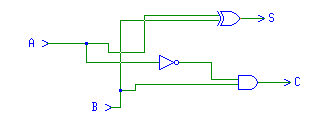
\includegraphics[width=0.8\linewidth]{HS}
			\centering
		 \end{figure}



		\subsubsection*{Análisis de resultados}
		El circuito funciona adecuadamente. Tiene el area y retraso de un CPA de 16bits.

\section{FASE 3: Sumadores CSA}
	\subsection{TAREA 9: Carry Select Adder}
		\subsubsection*{Especificación}
		Realizad el circuito digital sumador Carry Select Adder (CSA) de 4 bits que se muestra
		en la siguiente figura e indicad y formulad los tiempos de retardo y el área utilizada. Asumid el
		diseño de Carry Propagate Adder (CPA) de 4 bits implementado en la Tarea 4 y un retardo para el
		multiplexor de 3T. (0.75P)

		\begin{figure}[ht]
			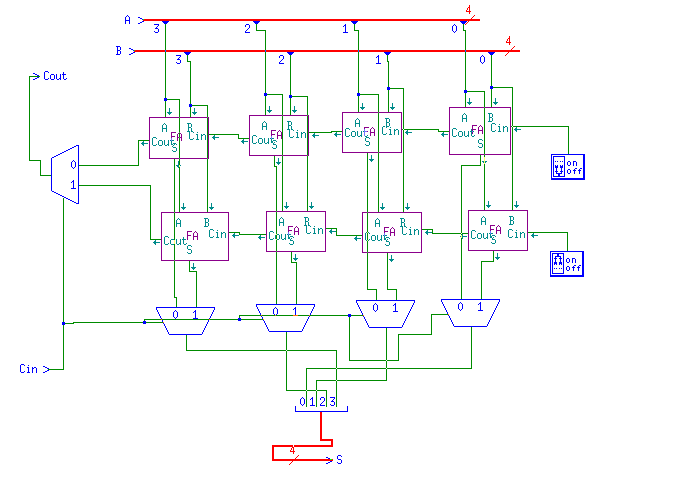
\includegraphics[width=0.8\linewidth]{CSA}
			\centering
		\end{figure}


		\subsubsection*{Diseño}
		Se ha implementado el circuito tal como se muestra en la imagen de ejemplo.


		\subsubsection*{Implementación}
		 \begin{figure}[ht]
		 	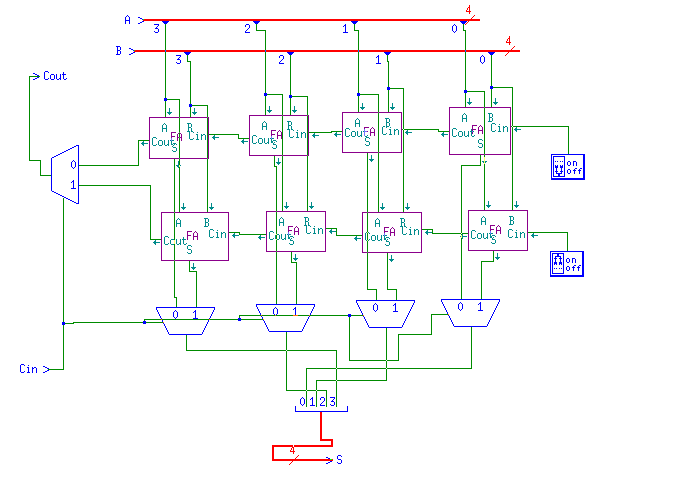
\includegraphics[width=0.8\linewidth]{CSA}
		 	\centering
		 \end{figure}


		\subsubsection*{Juego de pruebas}
		\begin{table}[h]
			\begin{center}
				\begin{tabular}{| c | c | c | c |}
					\hline
					Tipo de prueba & Operación & Resultado esperado & Funciona \\ \hline
				
					Suma & 3+2 Ci=1 & 6 Co=0 & Si \\ \hline
					Suma con carry & 7+8 Ci=1 & 0 Co=1 & Si \\ \hline
			
				\end{tabular}
				\caption Juego de pruebas
			\end{center}
		\end{table}



		\subsubsection*{Análisis de resultados}
		El circuito funciona adecuadamente. Tiene un área de 312 unidades y un tiempo de retardo de 40T del Carry y 37T en la suma.

	\subsection{TAREA 10: CSA de 16 bits}
		\subsubsection*{Especificación}
		Realizad un circuito digital Carry Select Adder (CSA) de 16 bits e indicad y formulad
		los tiempos de retardo y el área utilizada. Utilizad para esta implementación el circuito Carry Select
		Adder (CSA) de 4 bits implementado en una tarea anterior. (0.75P)


		\subsubsection*{Diseño}
		Se ha implementado el circuito tal como se muestra en la imagen de ejemplo.


		\subsubsection*{Implementación}
		 \begin{figure}[ht]
		 	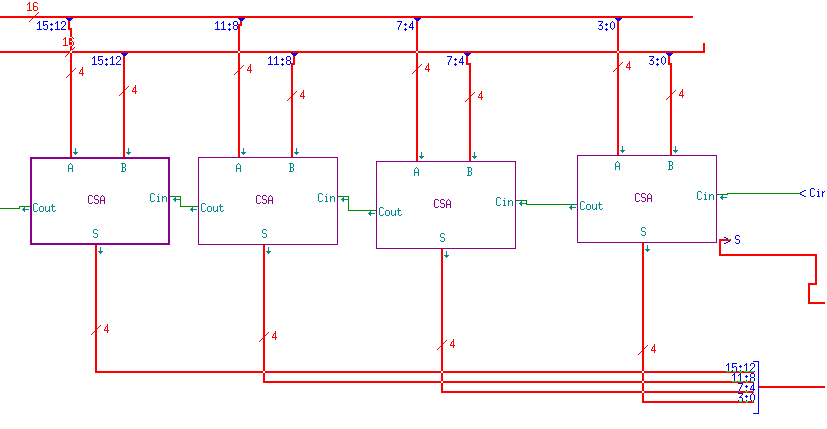
\includegraphics[width=0.8\linewidth]{CSA16}
			\centering
		 \end{figure}


		\subsubsection*{Juego de pruebas}
		\begin{table}[h]
			\begin{center}
				\begin{tabular}{| c | c | c | c |}
					\hline
					Tipo de prueba & Operación & Resultado esperado & Funciona \\ \hline
					
					Suma & 16+16 Ci=1 & 33 Co=0 & Si \\ \hline
					Suma con carry & 0xffff + 0xa & 9 Co=1 & Si \\ \hline
				\end{tabular}
				\caption Juego de pruebas
			\end{center}
		\end{table}



		\subsubsection*{Análisis de resultados}
		El circuito funciona adecuadamente. Tiene una área de 1248 unidades, y un tiempo de retardo de 46T del Carry y 43T de la suma.

\section{FASE 4: Sumadores CLA}
	\subsection{TAREA 11: Partial Full Adder}
		\subsubsection*{Especificación}
		Realizad el circuito digital Partial Full Adder (PFA) de 1 bit con acarreo de entrada
		que se muestra en la siguiente figura e indicad los tiempos de retardo y el área utilizada. Suponed
		que los retardos de las puertas lógicas utilizadas son de AND=4T, OR=4T y XOR=5T. (0.25P)


		\subsubsection*{Diseño}
		Se ha seguido el diseño mostrado en la imagen de ejemplo.

		\subsubsection*{Implementación}
		 \begin{figure}[ht]
			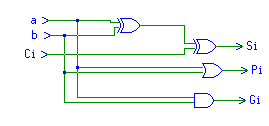
\includegraphics[width=0.8\linewidth]{PFA}
		 	\centering
		 \end{figure}


		\subsubsection*{Análisis de resultados}
		El circuito funciona adecuadamente. Tiene un área de 28 unidades y un tiempo de retardo de 10T para la suma y 4T para la propagación y la generación.

	\subsection{TAREA 12: Carry Look-Ahead Adder}
		\subsubsection*{Especificación}
		Realizad el circuito digital Carry Look-Ahead Adder (CLA) de 4 bits que se muestra en
la siguiente figura e indicad los tiempos de retardo y el área utilizada. Asumid el diseño de Partial
Full Adder (FA) de 1 bit implementado en la tarea anterior. Suponed que los retardos de las puertas
lógicas utilizadas son de AND=4T, OR=4T y XOR=5T. (0.75P)


		\subsubsection*{Diseño}
		Se ha seguido el diseño mostrado en la imagen de ejemplo. Se ha implementado el modulo lógico a parte para la tarea 13, incorporando las señales GG y PG.
		\subsubsection*{Implementación}
		 \begin{figure}[ht]
		 	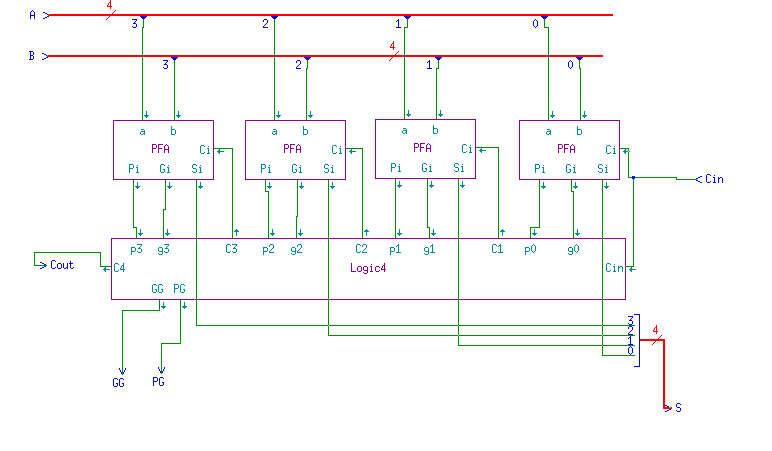
\includegraphics[width=0.8\linewidth]{CLA}
		 	\centering
		 \end{figure}
		
		 \begin{figure}[ht]
		 	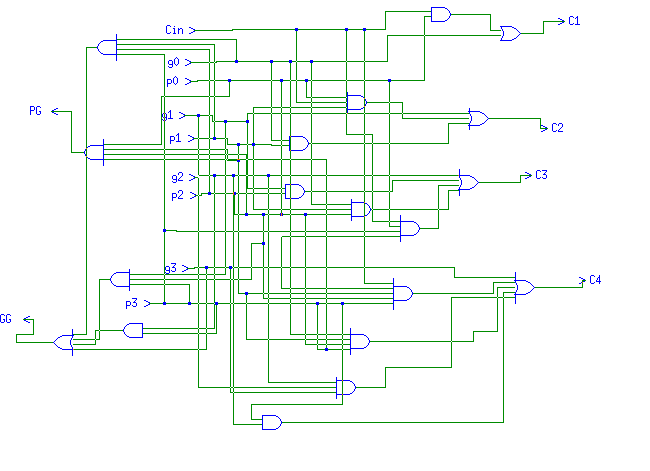
\includegraphics[width=0.8\linewidth]{CLALogic}
			\centering
		 \end{figure}


		\subsubsection*{Juego de pruebas}
		\begin{table}[h]
			\begin{center}
				\begin{tabular}{| c | c | c | c |}
					\hline
					Tipo de prueba & Operación & Resultado esperado & Funciona \\ \hline
				
					Suma & 3+2 Ci=1 & 6 Co=0 & Si \\ \hline
					Suma con carry & 7+8 Ci=1 & 0 Co=1 & Si \\ \hline
			
				\end{tabular}
				\caption Juego de pruebas
			\end{center}
		\end{table}



		\subsubsection*{Análisis de resultados}
		El circuito funciona adecuadamente. Tiene un área de 272 unidades y un tiempo de retardo de G y P de 4T, de los Carry a 8T, y 10T-5T ya que una XOR por una en paralelo, para un total de 17T.


	\subsection{TAREA 13: CLA de 16 bits}
		\subsubsection*{Especificación}
Realizad un circuito digital Carry Look-Ahead Adder (CLA) de 16 bits mediante los
CLA de 4 bits implementados en la tarea anterior y conectadlos en cascada tal y como se muestra en
la siguiente figura. Indicad los tiempos de retardo y el área utilizada. (0.75P)


		\subsubsection*{Diseño}
		Se ha implementado el circuito haciendo uso del modulo de la tarea anterior, el cual utiliza los Propagate y Generate generales para calcular estas señales en el circuito entero.


		\subsubsection*{Implementación}
		 \begin{figure}[ht]
			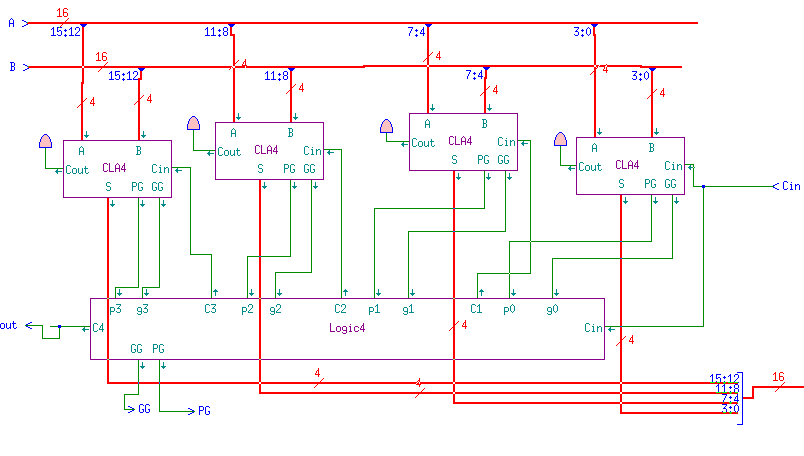
\includegraphics[width=0.8\linewidth]{CLA16}
		 	\centering
		 \end{figure}

		\subsubsection*{Análisis de resultados}
				El circuito funciona adecuadamente. Tiene un área de 1248 unidades y un tiempo de retardo de 8T para PG, 12T para PG, 30T para la suma y 25T para el carry.


	\subsection{TAREA 14}
		\subsubsection*{Especificación}
		Calculad los tiempos de retardo de todas las señales del circuito digital Carry Look-
		Ahead Adder (CLA) de 16 bits implementado en la tarea anterior. (1P)

		\subsubsection*{Análisis de resultados}
		Las señales p y g tienen 4T, mientras que PG y PP 12T. S0 tiene 10T, y de S1..S3 17T. De C1..C3 12 T. C4 son 16T. C8,12,16 20T. C9..C11,C13..C15 tiene 25T. S4 tiene 21T. S5..S7 26T. S8, S12 25T, y S9..S11,S13..S15 30T.

	\subsection{TAREA 15: Comparación entre CPA, CSA y CLA}
		\subsubsection*{Especificación}
		Comparad los tiempos y áreas de los sumadores Carry Propagate Adder (CPA), Carry Save Adder (CSA) y Carry Look-Ahead Adder (CLA) de 16 bits realizados anteriormente.

		\subsubsection*{Análisis de resultados}
		El CPA tiene el mayor tiempo de retardo, debido al problema de la propagación del carry, pero es el más eficiente en terminos de espacio. El CLA es el más rápido, pero tiene el mayor coste espacial. El CSA tiene un equilibrio entre espacio y tiempo de retardo. 
		En una situación realista, lo más probable es que querramos tener la mayor velocidad posible, ya que el espacio no suele ser un problema, así que elegiriamos el CLA.
\section{FASE 5: Multiplicador RCA}

	\subsection{TAREA 16}
		\subsubsection*{Especificación}
		Realizad un circuito digital multiplicador Riple Carry Array de 2 bits e indicad los
		tiempos de retardo y el área utilizada. Asumid el diseño de Half Adder (HA) implementado en una
		tarea anterior y un retardo para las puertas AND de 4T. (0.5P)

		\subsubsection*{Diseño}
		Se ha implementado una versión reducida del circuito de 4 bits utilizando puertas AND y HA. Para esta implementación no se requieren de FA.
		\subsubsection*{Implementación}
		 \begin{figure}[ht]
		 	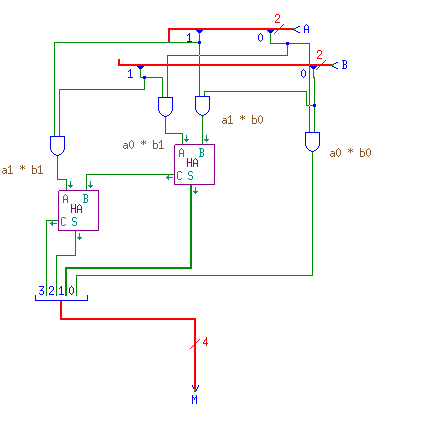
\includegraphics[width=0.8\linewidth]{RCA2}
		 	\centering
		 \end{figure}

		\subsubsection*{Análisis de resultados}
		Tiene un area de 52T. El camino crítico de este multiplicador le da un retardo máximo de 13T.
	\subsection{TAREA 17: Ripple Carry Array}
		\subsubsection*{Especificación}
		Realizad el circuito digital multiplicador Riple Carry Array de 4 bits que se muestra en
		la siguiente figura e indicad el tiempo de retardo y el área utilizada. Asumid los diseños de Half
		Adder (HA) y Full Adder (FA) de 1 bit implementados en las tareas anteriores. Suponed también
		que los retardos de las puertas lógicas utilizadas son de AND=4T, OR=4T y XOR=5T. (1P)

		\begin{figure}[ht]
			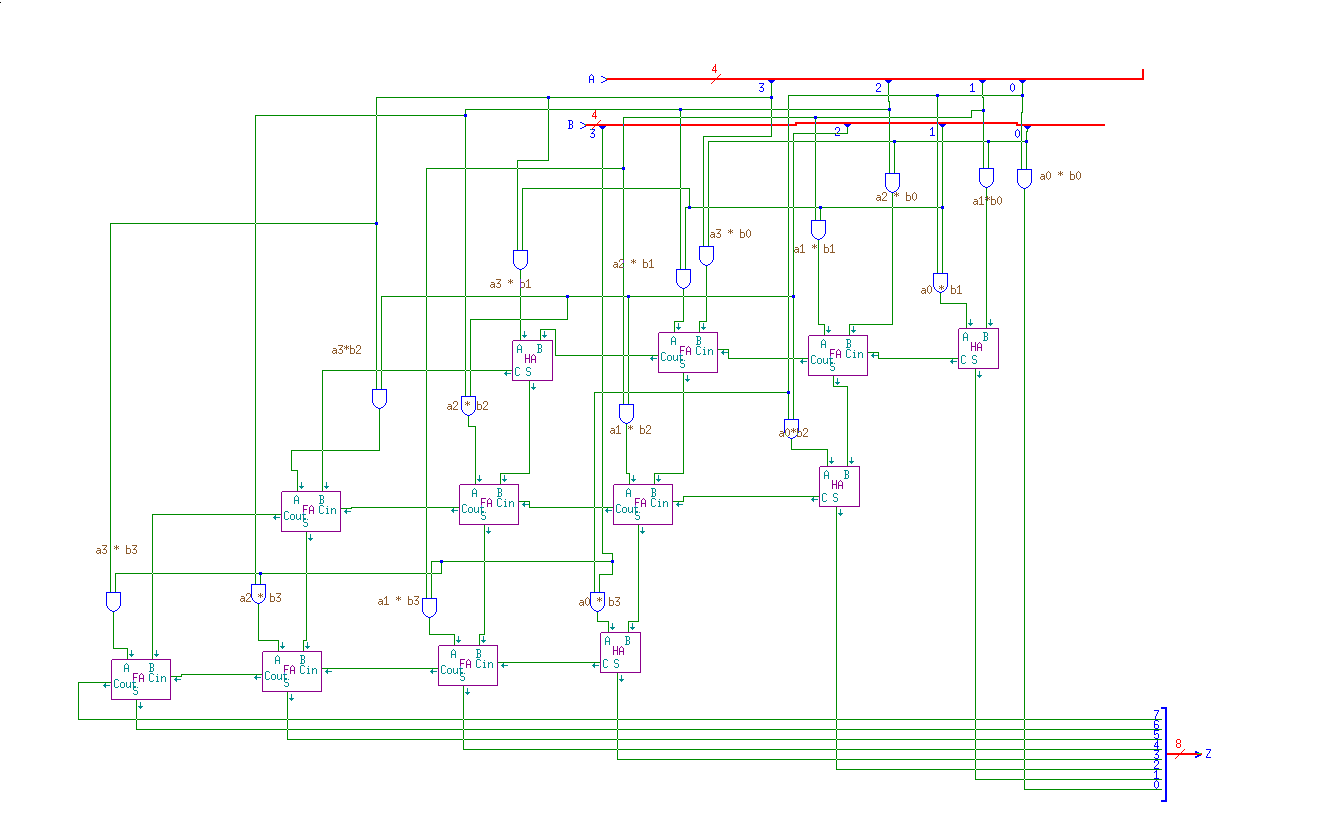
\includegraphics[width=0.8\linewidth]{RCA4}
			\centering
		\end{figure}


		\subsubsection*{Diseño}
		Se han usado los HA y FA de la tarea 1. Para crear el circuito, se ha seguido el diseño de la figura.


		\subsubsection*{Implementación}
		 \begin{figure}[ht]
		 	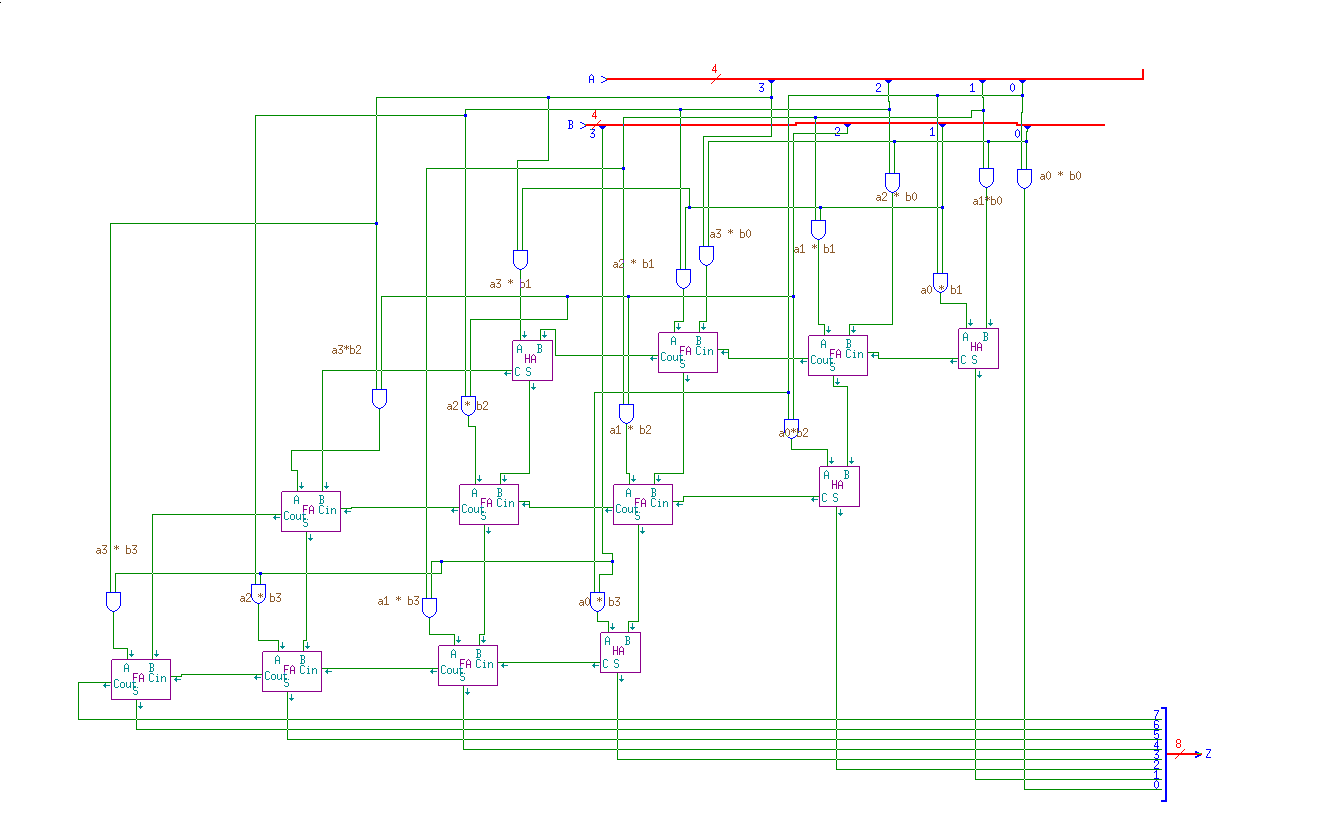
\includegraphics[width=0.8\linewidth]{RCA4}
		 	\centering
		 \end{figure}


		\subsubsection*{Juego de pruebas}
		Se han comprobado diferentes combinaciones de entradas $X,Y$ (multiplicadas entre sí): $0, 1, 2, 3, 4, 10, 15$ y todas dan el resultado $Z$ esperado.


		\subsubsection*{Análisis de resultados}
		Tiene un area de 424 y un retardo de 65T.
	\subsection{TAREA 18}
		\subsubsection*{Especificación}
		Calculad los tiempos de retardo de todas las señales del circuito circuito digital
		multiplicador Riple Carry Array de 4 bits implementado en la tarea anterior. (0.5P)
		\subsubsection*{Análisis de resultados}
		\begin{figure}[ht]
			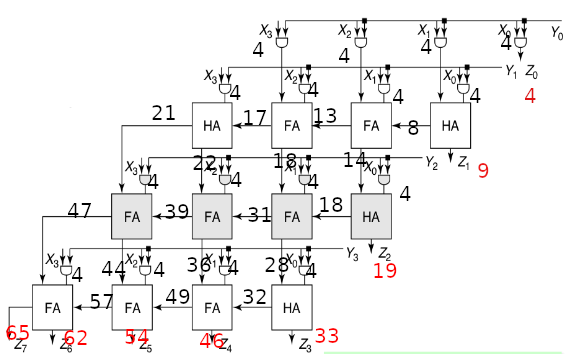
\includegraphics[width=0.8\linewidth]{RCA_RETARD}
			\centering
		\end{figure}

\end{document}
